\section*{Introduction}
\begin{frame}
    \frametitle{Wtf is Linux ?}
        \begin{itemize}
            \item Linux is a \textbf{Kernel} not an \textbf{Operating System}
            \item It was released in 1991 by Linus Torvalds, his work is based on MINIX
            \begin{itemize}
                \item Tanenbaum-Torvalds debate
            \end{itemize}
            \item Most of Linux based OSes are often built with a GNU Userland
            \begin{itemize}
                \item This is called a distribution, there are a lot of GNU/Linux distros (Debian, Ubuntu, Slackware, Archlinux, Gentoo, etc.)
                \item We are lazy, so we will say 'Linux'
            \end{itemize}
            \item Linux based OSes are UNIX-like OSes
        \end{itemize}
\end{frame}

\begin{frame}
        \begin{center}
            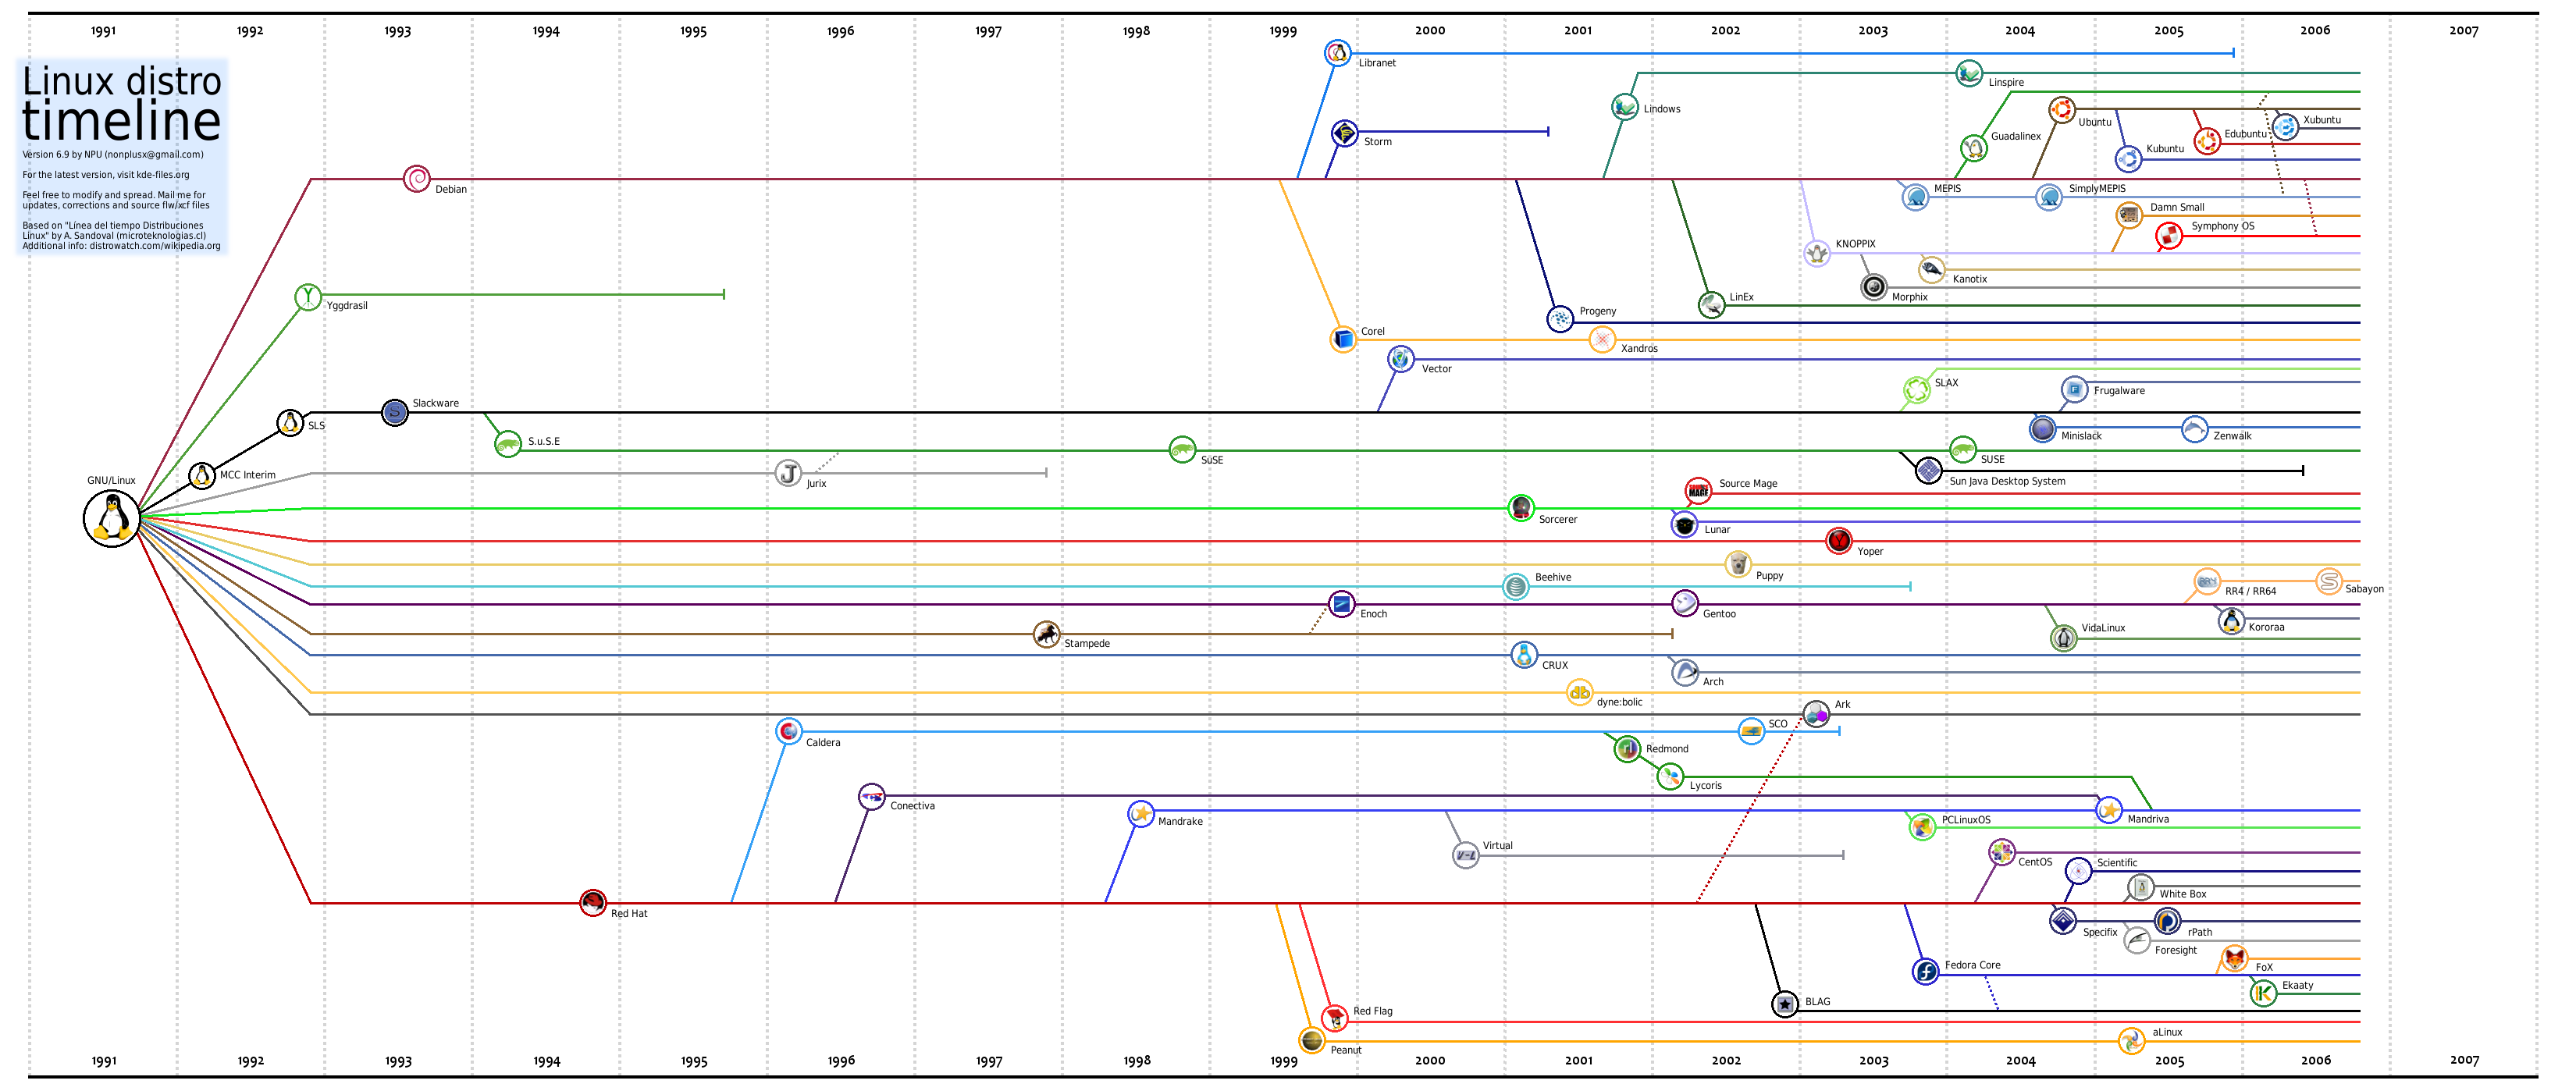
\includegraphics[scale=0.1]{linux_timeline.png}
        \end{center}
\end{frame}
